\begin{savequote}[45mm]
Quantization is an art form which, when applied to classical physical theories, yields predictions of subatomic behavior which are in spectacular agreement with experiments. 
\qauthor{Ron Y. Donagi}
\end{savequote}
\chapter{Canonical Quantization}
\section{What is Canonical Quantization}
Canonical Quantization is a tool or a set of mathematical formulations that enables us to transform a classical field into a quantum field by quantizing it. 
In developing canonical quantization we’ll see that particles are added or removed from a system  using field operators and these are formed from the creation and annihilation operators. 
\subsection{How is it done?}
Canonical quantization is done by following a set of processess which enables us to quantize a specific classical field of our choice. They are as follows, 
\begin{enumerate}[I]
    \item Writing down a classical Lagrangian density in terms of fields. This is the most tricky part as there are many possible lagrangians.  
    \item Calculating the momentum density and the Hamiltonian density in terms of fields.
    \item Now consider the fields and momentum density as operators. Pen down the commutation relations on them to make them quantum mechanical.
    \item Expand the fields in terms of creation/annihilation operators.
This will allow us to use occupation numbers and thereby making our job easier. 
  \item Now we have a quantum field considering the fact that we know the normal ordering interpretation. 
\end{enumerate}
\subsection{An Example}
Now lets say we have our Lagrangian for the scalar field at hand. Let's consider the Lagrangian for a massive scalar field given by, 
\begin{equation}
    L = \frac{1}{2} [\delta _{\mu} \phi(x) ]^{2} - \frac{1}{2} m^{2} [\phi(x)]^{2}
 \end{equation}
 The Klein-Gordon equation for this is given by,  $(\delta^{2}+m^{2})\phi = 0$ leading to a dispersion of $E_{p} = p^{2} + m^{2}$. \\
 \\
 Next we find the momentum density, 
 \begin{equation}
     \Pi^{\mu} (x) = \frac{\delta L}{\delta (\delta _{\mu} \phi(x))} 
 \end{equation}
 The time-like component of this tensor is $\Pi^{0}(x)= \pi{x}= \delta^{0} \phi(x)$. This helps us to determine the Hamiltonian in terms of momentum density. 
 \begin{equation}
     H = \Pi^{0}(x)\delta_{0}\phi(x) - L
 \end{equation}
 And now using our Lagrangian, we get the Hamiltonian density, 
 \begin{gather}
     H = \delta^{0} \phi(x) \delta_{0}\phi(x) - L  \\
     = \frac{1}{2} [\delta_{0} \phi(x)]^{2} + [\frac{1}{2} \nabla \phi(x)]^{2} +[\frac{1}{2} m^{2}\phi(x)]^{2}
 \end{gather} 
 We now turn the fields into field operators. We take $\phi(x) -> \hat{\phi}(x)$ and $\Pi^{0}(x) -> \hat{\Pi^{0}}(x)$. To make these field operators quantum mechanical we need to formulate the commutation relations between them. We impose the commutation relation by using the analogous commutation relations that we have in Quantum Mechanics.($[\hat{x}, \hat{p}] = i \hbar $)
 \begin{equation}
     [\hat{\phi}(t,x), \hat{\Pi}^{0}(t,y)] = i \delta ^{(3)} (x,y)
 \end{equation} 
 We also have ,
 \begin{equation}
     [\hat{\phi}(x),\hat{\phi}(y) ] = [\hat{\Pi}^{0}(x), \hat{\Pi}^{0}(y)] = 0 
 \end{equation} 
 This also applies to their dagger versions. \\
 Now the next and the most essential part is where we try to represent all the operators in terms of the annihilation and creation operators. Doing this makes our job very easy and comfortable to work with. \\
 In the case of Coupled oscillators, we have seen that, 
 \begin{equation}
     \hat{x}_{j} = (\frac{h}{m})^{\frac{1}{2}} \sum_{k} \frac{1}{(2 \omega_{k} N )^{\frac{1}{2}}} (\hat{a}_{k}e^{ijka} + \hat{a}^{\dagger}_{k}e^{-ijka}) 
 \end{equation}
 with $E_{p}= (p^{2}+m^{2})$
 In analogy to this, we write down a time-independent field operator for the continuous case as, 
 \begin{equation}
     \hat{\phi}(x) = \int\frac{d^{3}p}{(2\pi)^{\frac{3}{2}}} \frac{1}{(2 E_{p})^{\frac{1}{2}}} (\hat{a}_{p}e^{ip \cdot x} + \hat{a}^{\dagger}_{p}e^{-ip \cdot x})
 \end{equation}
 The commutation relation between the creation and annihilation operators is given by, 
 \begin{equation}
     [\hat{a}_{p}, \hat{a}^{\dagger}_{q}] = \delta^{(3)}(p-q)
 \end{equation}
 To obtain the time dependence on the above equation, we use the Heisenberg interpretation, 
 \begin{equation}
     \hat{\phi}(x) = \hat{\phi}(t,x) = \hat{U}^{\dagger}(t,0) \hat{\phi}(x) {U}^{\dagger}(t,0) = e^{i \hat{H}t} \hat{\phi}(x) e^{-i \hat{H}t}
 \end{equation}
 The creation and annihilation operators act only on $\hat{U}(t,0)$ and hence, 
 \begin{equation}
     \hat{U}^{\dagger}(t,0) a_{p} \hat{U}(t,0) = e^{iE_{p}t} \hat{a}_{p}
 \end{equation}
 This tells us that $\hat{a}_{p}$ picks up at $ e^{-iE_{p}t}$ and $\hat{a}^{\dagger}_{p}$ at $ e^{iE_{p}t}$ \\
 Equation (6.9) is called the mode expansion equation, which we will be covering the upcoming chapters in this section.
 \section{Justifying the Normalizing Factors}
 Now that we've established the mode expansion equation, the unsettling thing that we happen to see is the appearence of random constants in the equation. In this section, let's see how does one arrive at the constants present in that equation. \\
 In the aforementioned integral (equation 6.9),  we see that the momentum term "$d^{3}p$" is not a Lorentz-invariant quantity. We can also use the four momentum representation "$d^{4}p$" where $p= (p^{0}, p)$, but only those values of momenta should be considered for which $p^{2} = m^{2}$. This condition or a constraint is called the \textbf{"Mass shell condition"}
 \begin{figure}[h!]
     \centering
     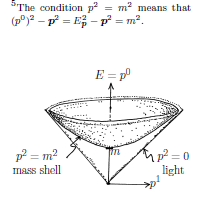
\includegraphics{Figures/massshell.png}
     \caption{Mass Shell}
     \label{fig:my_label}
 \end{figure}
 We write the momentum part as, 
 \begin{equation}
     d^{4}p \: \delta (p^{2}- m^{2}) \theta(p^{0})
 \end{equation}
 Where $\theta(p^{0})$ is called the Heaviside step function. It gives 0 for negative values and 1 for positive values of the function. We use this as we always require the positive values for the above relation. \\
  The Lorentz invariant for this can be written as, 
  \begin{equation}
      \frac{d^{3}p}{(2\pi)^{3}2 E_{p}}
  \end{equation}
  We have included $\frac{1}{(2\pi)}$ for every component of the thee momentum, as the mode expansion is essentially  a reverse fourier transform. \\
  We can normalise the integral by, 
  \begin{equation}
      1= \int \frac{d^{3}p}{(2\pi)^{3}2 E_{p}} \ket{p} \bra{p}
  \end{equation}
  We previously normalized momentum states as $\bra{p}\ket{q}= \delta ^{3}(p-q)$. Hence the four momentum state can be written in terms of the three momentum state as, 
  \begin{equation}
      \ket{p}= (2\pi)^{\frac{3}{2}}(2E_{p})^{\frac{1}{2}} \ket{p}
  \end{equation}
  The new normalization can be written as, 
  \begin{equation}
      \bra{p}\ket{q} = (2\pi)^{3}(2E_{p}) \delta^{(3)} (p-q)
  \end{equation}
  We can define the creation operator $\alpha$ as, 
  \begin{equation}
      \hat{\alpha}^{\dagger}_{p} = (2\pi)^{\frac{3}{2}}(2E_{p})^{\frac{1}{2}} \hat{a}^{\dagger}_{p}
  \end{equation}
  
  Hence our integral becomes, 
  \begin{equation}
       \hat{\phi}(x) = \int\frac{d^{3}p}{(2\pi)^{3}} \frac{1}{(2 E_{p})} (\hat{\alpha}_{p}e^{ip \cdot x} + \hat{\alpha}^{\dagger}_{p}e^{-ip \cdot x})
  \end{equation}
  Now in terms of $\hat{a}^{\dagger}_{p}$ and $ \hat{a}_{p}$, the integral can be rewritten as, 
  \begin{equation}
      \hat{\phi}(x) = \int\frac{d^{3}p}{(2\pi)^{\frac{3}{2}}} \frac{1}{(2 E_{p})^{\frac{1}{2}}} (\hat{a}_{p}e^{ip \cdot x} + \hat{a}^{\dagger}_{p}e^{-ip \cdot x})
  \end{equation}
 \section{What about the Hamiltionian?}
 Now by substituting the expansion of the field operator $\hat{\phi}(x)$ in the hamiltonian equation in terms of the creation and annihilation operators, we get, 
 \begin{equation}
     \hat{H} = \int d^{3}x \frac{1}{2} ([\delta_{0}\phi(x)]^{2} +   [\nabla \phi(x)]^{2} +[ m^{2}\phi(x)]^{2})  
 \end{equation}
 Now we substitute this in the mode expansion equation and use the commutation relations to simplify it. The momentum density calculated is $\hat{\Pi}_{\mu}(x) = \delta _{\mu} \hat{\phi}(x) $ which is given by, 
 \begin{equation}
     \hat{\Pi}_{\mu} = \delta _{\mu} \hat{\phi}(x) =  \int\frac{d^{3}p}{(2\pi)^{\frac{3}{2}}} \frac{1}{(2 E_{p})^{\frac{1}{2}}} (-ip_{\mu}) (\hat{a}_{p}e^{ip \cdot x} + \hat{a}^{\dagger}_{p}e^{-ip \cdot x})
 \end{equation}
 To obtain $\delta _{0} \hat{\phi}(x)$,  we consider only the time-like component of the momentum density. 
 \begin{equation}
     \delta _{0} \hat{\phi}(x) = \int\frac{d^{3}p}{(2\pi)^{\frac{3}{2}}} \frac{1}{(2 E_{p})^{\frac{1}{2}}} (-iE_{p}) (\hat{a}_{p}e^{ip \cdot x} + \hat{a}^{\dagger}_{p}e^{-ip \cdot x})
 \end{equation}
 The space-like components of the momentum density gives us $\nabla \hat{\phi}(x)$, 
 \begin{equation}
     \nabla \hat{\phi}(x) = \int\frac{d^{3}p}{(2\pi)^{\frac{3}{2}}} \frac{1}{(2 E_{p})^{\frac{1}{2}}} (ip) (\hat{a}_{p}e^{ip \cdot x} + \hat{a}^{\dagger}_{p}e^{-ip \cdot x})
 \end{equation}
 Now we have all the necessary factors to compute the hamiltonian. 
 \begin{equation}
     E = \int d^{3} p E_{p} (\hat{a}^{\dagger}_{p}\hat{a}_{p} + \frac{1}{2}\delta^{3}(0))
 \end{equation}
 The last term in the above expression must seem daunting. It leads the above integral to result in infinity. Although we will be working with the difference in the energy levels in which case the term $\frac{1}{2}\delta^{3}(0)$ will cancel out each other. But in terms of the individual expression the equation does not seem to make sense. We need to find a way to device a more reasonable expression in order to get rid of the infinity. The next section will cover the method through which we can deal with this problem.
 
 
 
 
 
 
 
 
 
 
 
 
\section{Normal Ordering}
The infinity that we just encountered is due to the  ambiguity in the Lagrangian. Let's consider a general classical theory formed from complex values fields $\psi(x)$. The Lagrangian describing these fields will contain bilinear terms like $\psi^{\dagger}\psi$ (as we require the Lagrangian to be $\in \mathbb{R}$), which could equally well be written in a classical theory as $\psi\psi^{\dagger}$. However, when we quantize the order that was chosen suddenly becomes crucial. So we undergo a process called \textbf{"Normal ordering"} which removes the ambiguity to give a meaningful quantum theory. We simply need to arrange the operators in a way so that all the creation operators are placed in the left \\
\begin{figure}[!ht]
	\centering
	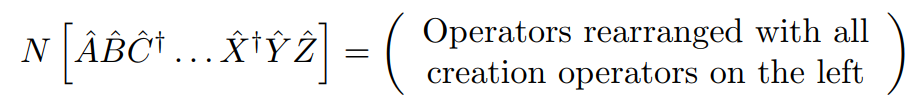
\includegraphics[scale=0.5]{Figures/NormalOrd.png}
	%\caption{A Plot of $\delta(x)$}
\end{figure}
Here $N$ is called the "normal ordering operator", although it doesn't act on states in the traditional sense. When we rearrange operators: there is nothing strange going on for Bose fields, however we do pick up a ${(-1)}^{P}$ (where $P$ is the number of permutations needed to normally order a product of operators) factor when we normally order the product on the left.
Now let's get back to the Hamiltonian, With the normal ordering interpretation the old expression
\begin{equation}
    \hat{H}  = \frac{1}{2} \int d^{3}p \ E_{p}(\hat{a}_{p}\hat{a}^{\dagger}_{p} + \hat{a}^{\dagger}_{p}\hat{a}_{p})
\end{equation}
then becomes
$$N[\hat{H}] = \frac{1}{2} = \int d^{3}p \ E_{p} \ N[\hat{a}_{p}\hat{a}^{\dagger}_{p} + \hat{a}^{\dagger}_{p}\hat{a}_{p}]$$
$$N[\hat{H}] = \frac{1}{2} = \int d^{3}p \ E_{p} \ 2\hat{a}^{\dagger}_{p}\hat{a}_{p}$$
\begin{equation}
     N[\hat{H}] = \int d^{3}p \ E_{p} \ \hat{n}_{p}
\end{equation}
where $\hat{n}_{p} = \hat{a}^{\dagger}_{p}\hat{a}_{p}$ is the number operator. Acting on a state it tells you
how many excitations there are in that state with momentum p.
We now have a Hamiltonian operator that makes sense. 
What we seen now, is that the excited states of the wave equation
can be thought of as particles possessing quantized momenta. These
particles could be called scalar phions after the greek letter Phi ($\phi$) we use to denote the scalar field. They are Bosons with spin $0$. Similarly for spin $1/2$ particles we use spinors and vectors for spin $1$ particles.
\begin{tcolorbox}
\subsection{The Casimir Effect}
Consider two metal plates I and II separated by a distance $L$. We put a third
plate (III) in between them, a distance $x$ from plate I. 
\begin{figure}[!ht]
	\centering
	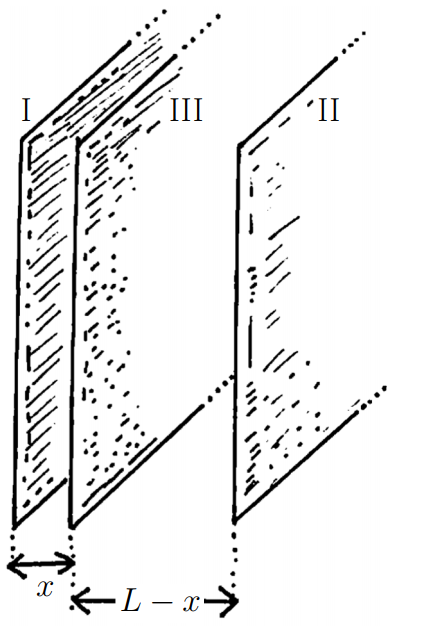
\includegraphics[scale=0.5]{Figures/Casimir.png}
	\caption{A schematic of the Casimir setup}
\end{figure}
We will derive the force on plate III resulting from the field on either side of it. The presence of the plates forces the field to be quantized according to $k_{n} = n \pi/x$ or $n\pi/(L − x)$. The
dispersion is $E_{n} = k_{n}$ and so the total zero-point energy is given by
\begin{equation}
    E = \sum_{n= 1}^{\infty} \left[\frac{1}{2} \left( \frac{n \pi}{x} \right) + \frac{1}{2} \left( \frac{n \pi}{L - x} \right)\right]
\end{equation}
that is, $1/2\hbar \omega_{n}$ per mode as for photons $\omega_{n} = ck_{n}$, and the zero-point energy is $1/2\hbar \omega_{n}$, so in
units in which $\hbar = c = 1$ this becomes
$1/2k_{n}$, and so $E = \sum_{n} 1/2k_{n}$. These sums both diverge, just as we expect since we are evaluating the infinite vacuum energy.
However, real plates can’t reflect radiation of arbitrarily high frequency: the highest energy modes leak out. To take account of this we cut off these high-energy modes
thus:
\begin{equation}
    \frac{n \pi}{2x} \rightarrow \frac{n \pi}{2x}e^{-n \pi a/x}
\end{equation}
We can thus now work out the sums,
$$f(x) = \sum_{n} \frac{n \pi}{2x} e^{-n \pi a/x}$$
$$f(x) = \frac{1}{2} \frac{\partial}{\partial a} \sum_{n}  e^{-n \pi a/x}$$
$$f(x) = \frac{1}{2} \frac{\partial}{\partial a} \frac{1}{1 - e^{n a/x}}$$
\begin{equation}
    f(x) = \frac{\pi}{2x} \frac{\partial}{\partial a} \frac{e^{n a/x}}{{(1 - e^{n a/x})}^{2}} \approxeq \frac{x}{2 \pi a^{2}} - \frac{\pi}{24x} + O(a^{2})
\end{equation}
The total energy between I and II is 
\begin{equation}
    E = f(x) + f(L -x) = \frac{L}{2 \pi a^{2}} - \left(\frac{1}{x} - \frac{1}{L-x}\right) + O(a^{2})
\end{equation}
And if $x << L$, we find a force
\begin{equation}
    F = -\frac{\partial E}{\partial x} = -\frac{\pi}{24 x^{2}}
\end{equation}
which is independent of $a$, as we hoped. Thus, there is an attractive force between
the closely spaced plates I and III. This is the Casimir force. We can understand
this force intuitively by realizing that as the two plates are pulled together we lose
the high-energy modes. This reduces the energy between the plates and leads to
an attractive force. A more quantum-field-theory friendly interpretation is that the
effect results from quantum fluctuations in the vacuum, in which particles are spontaneously created and annihilated
\end{tcolorbox}

\section{Deciphering the Mode Expansion}

However if we recall the Klein-Gordon equation, it had two different solutions. One corresponding to incoming particles and the other to outgoing anti-particles. We can't just
\begin{figure}[!ht]
	\centering
	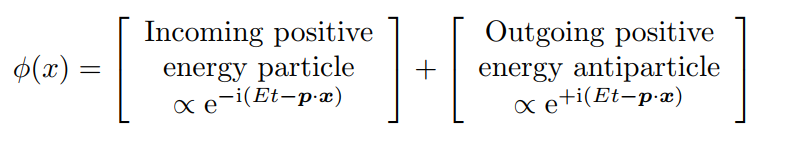
\includegraphics[scale=0.5]{Figures/anti.png}
	\caption{Feynman's interpretation of the solutions to the Klein-Gordon equation}
\end{figure}
The expansion is carried out in terms of incoming plane waves $e^{−ip·x}$.Incorporating Feynman's picture, incoming here means, not only a factor
$e^{−ip·x}$, but also that the particle is annihilated: it comes into the system
and is absorbed by it. Conversely, outgoing means a factor $e^{ip·x}$ and
that the particle is created. We therefore interpret the mode expansion as
\begin{figure}[!ht]
	\centering
	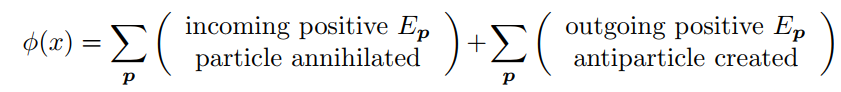
\includegraphics[scale=0.5]{Figures/Parts.png}
	\caption{Interpreting the modified mode expansion}
\end{figure}
The resulting expansion of a field annihilation operator is
\begin{equation}
    \hat{\phi} = \int \frac{d^{3}p}{{(2 \pi)}^{3/2}} \frac{1}{{2 E_{p}}^{1/2}} (\left \hat{a}_{p}e^{-i.px} + \hat{b}^{\dagger}_{p}e^{i.px} \right)
\end{equation}
\section{An Example: Complex Scalar Field Theory}
\subsection{Canonically quantizing the Scalar field}
For complex scalar fields, there are two components, $\psi(x) and (\psi^\dagger(x))$. We need to canonically quantize the Lagrangian using the procedure we saw before.
The Lagrangian for the complex scalar field theory is,
\begin{equation}
    \mathcal{L}=\partial^{\mu}\psi^\dagger(x)\partial_\mu\psi(x)-m^2\psi^\dagger(x)\psi(x)
\end{equation}




\section{The Trouble With Canonical Quantization}
Despite it's outlook, canonical quantization does not work for all theories. It only holds for Lagrangians which cannot be written in terms of quadratic parts composed of it's field and derivatives. The result of canonical quantization is a system described by single particles in momentum states which don’t interact with each other. We refer to the Lagrangians which can be canonically quantized as \textbf{non-interacting theories} and it's opposites as \textbf{interacting theories}. Moreover some have criticized it on being non-fundamental and ad-hoc.

\epigraph{Already from first principles one encounters difficulties. Given that the classical description of a system is an approximation to its quantum description, obtained in a macroscopic limit (when $\hbar \rightarrow 0$), one expects that some information is lost in the limit. So quantization should somehow have to compensate for this. But how can a given quantization procedure select, from amongst the myriad of quantum theories all of which have the same classical limit, the physically correct one?}{\textit{Mac Flecknoe \\ John Dryden}}
